\documentclass{article}
%\documentclass[conference]{IEEEtran}
\usepackage[utf8]{inputenc}
\usepackage[english]{babel}
\usepackage{ragged2e}
\usepackage{blindtext}
\usepackage{geometry}
\usepackage{authblk}
\usepackage{comment}
\usepackage{rotating}
\usepackage{float}
\usepackage{amsmath}
\usepackage{amsfonts}
\usepackage{booktabs}
\usepackage{pifont}
\usepackage{amssymb}
\usepackage{algpseudocode}
\usepackage{scrextend}
\usepackage{caption}
\usepackage{subcaption}
\usepackage{threeparttable}
\usepackage{multicol}
\usepackage{lipsum}
\usepackage{booktabs, caption, makecell}
\usepackage{multirow}
\usepackage{tabularx}
\usepackage{graphicx}
\usepackage{subfigure}
\usepackage{biblatex}
\setlength{\columnsep}{1cm}


 \geometry{
 a4paper,
 total={170mm,257mm},
 left=20mm,
 top=20mm,
 }

\title{\huge \textbf{Domain Prompt Learning for Efficiently Adapting CLIP to Unseen Domains}\\

}
% Authors
\author[1]{\textbf{ Xin Zhang}}
\author[1,2]{\textbf{Shixiang Shane Gu} }
\author[1]{\textbf{Yutaka Matsuo}}
\author[1]{\textbf{Yusuke Iwasawa}}


\begin{comment}
\author{%
  Author 1\\Affilation 1
  \and Author 2\\Affiliation 2
  \and Author 3\\Affiliation 3
 
}    
\end{comment}


% Author Affiliations
\affil[1]{The University of Tokyo}
\affil[2]{Google Research, Brain Team}
\date{}


\renewenvironment{abstract}
 {\par\noindent\textbf{\abstractname}\ \ignorespaces}
 {\par\medskip}

\addbibresource{bib.bib} 
\begin{document}
\maketitle



\begin{multicols}{2}

\begin{abstract}
\\Domain generalization (DG) is a difficult transfer learning
problem aiming to learn a generalizable model for unseen domains. Recent foundation models (FMs) are robust to many
distribution shifts and, therefore, should substantially improve the performance of DG. In this work, we study generic
ways to adopt CLIP, a Visual-Language Foundation Model,
for DG problems in image classification. While ERM greatly
improves the accuracy with bigger backbones and training
datasets using standard DG benchmarks, fine-tuning FMs
is not practical in many real-world situations. We propose
DPL (Domain Prompt Learning) as a novel approach for domain inference in the form of conditional prompt generation.
DPL achieved a significant accuracy improvement with only
training a lightweight prompt generator (a three-layer MLP),
whose parameter is of equivalent scale to the classification
projector in the previous DG literature. Combining DPL with
CLIP provides surprising performance, raising the accuracy
of zero-shot CLIP from 73.7% to 79.3% on several standard
datasets, namely PACS, VLCS, OfficeHome, and TerraIncognita. We hope the simplicity and success of our approach
lead to broader adoption and analysis of foundation models
in the domain generalization field. Our code is available at
https://github.com/shogi880/DPLCLIP
\end{abstract}

\section{\centering Introduction}

Pre-training large vision models using web-scale images is
an essential ingredient of recent success in computer vision. Fine-tuning pre-trained models, such as ResNet (He
et al. 2015) and Vision Transformer (ViT) (Dosovitskiy et al.
2020) is the most popular paradigm for many downstream
tasks. However, domain shifts pose a substantial challenge
in real-world scenarios for successfully transferring models.
Over the past decade, various studies on domain generalization (DG) have sought a systematic way to narrow the gap
between source and target domains (Zhou et al. 2021a; Wang
et al. 2021; Shen et al. 2021) aiming to build a model that
generalizes to unseen domains. Despite the significant work
on this front, machine learning systems are still vulnerable
to domain shifts even after using DG methods (Gulrajani and
Lopez-Paz 2020).
Large pre-trained vision-language models like Contrastive Language-Image Pre-Training (CLIP) are an emerging category of models showing great potential in learning

\begin{figure}[H]
         \centering
         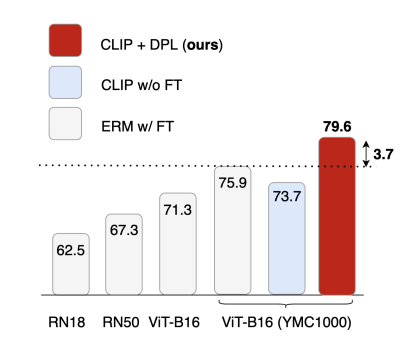
\includegraphics[width=0.5\textwidth]{1.png}
         \label{fig:three sin x}
         \caption{: Bigger backbone (from ResNet18 to ViT-B16) and
bigger pre-train dataset (from ImageNet to YMC1000) improve the performance of ERM on VLCS, PACS, OfficeHome, TerraIncognita. Even without fine-tuning the image
encoder, our DPL (Domain Prompt Learning) effectively
improves the performance of CLIP and outperforms the
baseline ERM by a large margin (3.7%). The CLIP w/o FT
use the template prompt, such as ‘a photo of a {class name}’.
}
\end{figure}

transferable representation across many vision tasks. At the
core of CLIP is to learn image representations by contrasting them with the representations of text description of the
image, such as ‘a photo of a {class name}’. The text description is often called prompt, and its design is vital in enhancing CLIP performance. Notably, CLIP can handle unseen
classes without fine-tuning them by adequately changing the
text description using the target class name.
This paper investigates the robustness of CLIP against
various distribution shifts using DomainBed (Gulrajani and
Lopez-Paz 2020), a recently proposed benchmark for DG
setup. While prior works test various DG methods in the
benchmark, the most studied only focused on medium-scale
pre-trained models, such as ResNet18 or ResNet50. There
are two na¨ıve approaches to leveraging CLIP in the DG
setup Figure 2. The first approach is fine-tuning the image encoder trained by CLIP, similar to the other vision models
such as ResNet and ViT. We show that the backbone networks trained by CLIP substantially outperform many backbone networks trained solely on images, such as ResNet,
big transfer (Kolesnikov et al. 2020), and vision transformer
(Dosovitskiy et al. 2020). At the same time, however, finetuning sometimes degraded the performance on some domains, suggesting that fine-tuning possibly distorts good
properties of pre-trained features (Kumar et al. 2022). Another na¨ıve approach is designing the template prompt, such
as ‘a photo of a {class name}’. The clear merit of this approach is that it does not require optimizing any network
and, therefore, keeps the representations learned via pretraining. Despite its simplicity, we show that zero-shot CLIP
is still more robust on many DG benchmarks than the vision
backbones (e.g., ResNet18, ResNet50, ViT-B16) fine-tuned
on source domains, while it is inferior to fine-tuning vision
backbone trained by CLIP.
Based on the observations, we propose Domain Prompt
Learning (DPL), a simple yet effective extension of CLIP
in the DG setup. A natural way to adapt the model is
to add domain-specific features to the prompt template.
However, manually designing a prompt template is challenging in many cases due to its ambiguity. Instead, we
propose DPL for automatically generating a prompt that
estimates domain-specific features given unlabeled examples from each distribution. More specifically, DPL trains a
lightweight prompt generator using source domains, which
outputs fixed-length continuous domain prompts given input
images of each distribution while freezing other networks.
During test-time, the prompt generator generates domain
prompt given input images from the target distribution and
adds them to the label prompts. Since the entire networks are
frozen, the core properties of the pre-training would remain
in DPL and are expected to improve CLIP performance in
DG stably, as shown in our experiments.
It is worth noting our work is not the first attempt to
tune the prompt of CLIP. For example, (Gao et al. 2021;
Zhou et al. 2021b) have proposed optimizing continuous
prompts on the target datasets, effectively improving CLIP
performance. CoCoOp (Zhou et al. 2022), as a contemporary
work, trains a meta-net to generate a meta token for adapting to each instance. CoCoOp focuses on unseen classes
and demonstrates its performance by transferring from ImageNet to the four specially designed ImageNet variants. This
work focuses on the robustness of CLIP against distribution shifts, and proposes a generic way to extract a domainspecific features and improve performance on the target domain at test-time.
We conduct experiments on four standard datasets included in DomainBed to evaluate DPL, following the experiment setup in(Gulrajani and Lopez-Paz 2020; Iwasawa and
Matsuo 2021), such as parameter tuning and model selection. We show that CLIP with DPL outperforms the strong
baselines by a large margin, raising the accuracy from 73.7%
to 79.6% (Table 1). Moreover, since DPL can be seen as a
kind of Test-Time Adaptation (TTA) method, we compare
it with a series of SoTA TTA methods and demonstrate the
efficiency of DPL (Table 2). And lastly, through various ab-lation studies, we surprisingly found that frozen backbone
outperforms fine-tuning on OfficeHome datasets for all of
ResNet, DeiT (Touvron et al. 2021), HViT, and ViT-B16 (Table 4). These results prove that DPL is effective, and more
importantly, they provide many insights for future works that
apply CLIP on DG.g
In summary, our main contributions are:
\begin{enumerate}
    \item We introduce CLIP to standard DG benchmark DomainBed via prompt learning.
    \item We propose Domain Prompt Learning (DPL), a novel approach of domain inference, to effectively help domain
generalization by utilizing domain-specific features.
    \item We demonstrate the impressive empirical performance of
DPL by comparing with strong DG baselines and a series
of state-of-the-art (SoTA) TTA methods.

\end{enumerate}
 



\begin{comment}
    \begin{center}
\captionof{table}{Arbitrary-length Text editing evaluation. We report FID
score and word-level recognition accuracy (\%). Although the supervised EditText can imitate more font category and background
texture, our self-supervised approach achieves better readability}
\begin{tabular}{ c c c c } 

 \hline
 Method & Supervision & FID & Acc. \\
 \hline
 EditText & \checkmark & \textbf{40.5} & 14.9 \\ 
 Ours & $\times$ & 67.9 & \textbf{57.6}  \\ 
 \hline
\end{tabular}
\end{center}
\end{comment}
\end{multicols}
\begin{figure}[H]
         \centering
         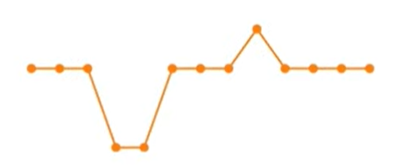
\includegraphics[width=0.8\textwidth]{2.png}
         \label{fig:three sin x}
         \caption{: Bigger backbone (from ResNet18 to ViT-B16) and
bigger pre-train dataset (from ImageNet to YMC1000) improve the performance of ERM on VLCS, PACS, OfficeHome, TerraIncognita. Even without fine-tuning the image
encoder, our DPL (Domain Prompt Learning) effectively
improves the performance of CLIP and outperforms the
baseline ERM by a large margin (3.7%). The CLIP w/o FT
use the template prompt, such as ‘a photo of a {class name}’.
}
\end{figure}
\begin{multicols}{2}
  

\section{\centering Method}
In this section, we first introduce the notations and definitions of DG following (Wang et al. 2021). Then, we explain how to use CLIP in DG and introduce Domain Prompt
Learning to enhance CLIP performance in DG

\subsection{ Problem Setup of DG}

\begin{equation}
    p_{ap}^{i} = 
    \frac{1}{N} = \sum_{j=1}^{N}F(f(x_{j}^{i}))
\end{equation}


\subsection{ Naıve Approaches for Using CLIP in DG}
\subsection{Domain Prompt Learning for CLIP in DG
}
\section{\centering Conclusion}
\subsection{Limitation}
\subsection{Future}

\lipsum[2]

\end{multicols}

\begin{table}[h!]
%\begin{threeparttable}
    \centering
    \caption{Multi col table}
    
    \begin{tabularx}{0.8\textwidth}{|c|c|c|c|}
        \hline
        \multirow{10}{*}{numeric literals} & \multirow{5}{*}{integers} & in decimal & 8743\\
        \hline
        & &  \multirow{2}{*}{in octal} & 7464\\
        \hline
        & & & 103\\
        \multirow{2}{*}{4}  & 5 & 6\\
        \cline{3-4}
        
        \hline
        \multicolumn{2}{|c|}{\multirow{2}{*}{10}} & 12\\
        \cline{3-3}
        \multicolumn{2}{|c|}{} & 17 \\
        \hline
        
    \end{tabularx}
    \begin{tablenotes}
      \item[1] Note that \textit{Getting On Sequence} will start from steady standing in the station.
      \item[2] Note that \textit{Getting Off Sequence} will start from steady sitting state in the Tram.
   \end{tablenotes}
    \label{tab:Multi col table}
    %\end{threeparttable}
\end{table}


\begin{equation}
    x = \frac{\sqrt{\sin{\theta}}+{\cos{\theta}}+T_i}{e^{-20}}
\end{equation}


\begin{equation}
    p_{ap}^{i} = 
    \frac{1}{N} = \sum_{j=1}^{N}F(f(x_{j}^{i}))
\end{equation}

\begin{figure}[H]
     \centering
     \begin{subfigure}[b]{0.4\textwidth}
         \centering
         \includegraphics[width=\textwidth]{1a.png}
         \caption{}
         \label{fig:y equals x}
     \end{subfigure}
     \begin{subfigure}[b]{0.4\textwidth}
         \centering
         \includegraphics[width=\textwidth]{1b.png}
         \caption{}
         \label{fig:three sin x}
     \end{subfigure}
     \begin{subfigure}[b]{0.4\textwidth}
         \centering
         \includegraphics[width=\textwidth]{1c.png}
         \caption{}
         \label{fig:five over x}
     \end{subfigure}
     \begin{subfigure}[b]{0.4\textwidth}
         \centering
         \includegraphics[width=\textwidth]{1d.png}
         \caption{}
         \label{fig:five over x}
     \end{subfigure}

        \caption{Schematic diagrams of SAINT and its various components. (a) Architecture of the self-attention module used in SAINT. (b) Architecture of the scaled dot-product attention sub-module. (c) Architecture of our proposed 2A3I module by augmenting self-attention within the 3I network. (d) A schematic diagram of the overall architecture of
SAINT, which comprises two 2A3I modules, three self-attention modules, convolutional layers with window size 11 and 2 dense layers}
        \label{fig:three graphs}

\end{figure}

\begin{comment}
\begin{center}
    \Large
    \textbf{Thesis Title}
        
    \vspace{0.4cm}
    \large
    Thesis Subtitle
        
    \vspace{0.4cm}
    \textbf{Author Name}
 
    \vspace{0.9cm}
    \begin{flushleft}
    \textbf{Abstract}
    \item[\textbf{Motivation :}]
    \item[\textbf{Results :}]
    \end{flushleft}
\end{center}
\end{comment}
\begin{multicols}{2}

\pagebreak
\begin{figure}[H]
         \centering
         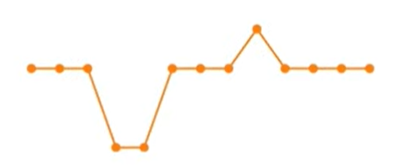
\includegraphics[width=0.5\textwidth]{2.png}
         \label{fig:three sin x}
         \caption{Accuracy of SAINT-base and MUFOLD-SS under various levels of non-local interactions. We show the results on the TEST2016 test set using six bins of proteins}
\end{figure}
\begin{figure}[H]
         \centering
         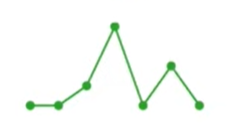
\includegraphics[width=0.5\textwidth]{3.png}
         \label{fig:three sin x}
         \caption{. Accuracy of SAINT, SPOT-1D, NetSurfP-2.0 and MUFOLD-SS as a function of the average number of non-local interactions per residue. We show the results on the six bins as shown in Table 6}
\end{figure}

\begin{comment}
    \begin{wrapfigure}{l}{0.25\textwidth}
\includegraphics[width=0.9\linewidth]{overleaf-logo} 
\caption{Caption1}
\label{fig:wrapfig}
\end{wrapfigure}
\end{comment}


\end{multicols}
\section{Bibliography}
We used info from \cite{arjovsky2019invariant}
\printbibliography


\end{document}
